\subsection{高信頼データ転送}

高信頼データ転送(reliable data transmission)
\begin{itemize}
  \item 誤り (0, 1の反転) がなく、かつ、送信された順序通りに届く
  \item エンド-エンドの制御でどうやって実現するのか
  \begin{itemize}
    \item[$\Rightarrow$] \textcolor{orange}{ARQ (Automatic Repeat reQuest)} プロトコルによる制御
    \item 誤り検知・送達確認を行いながら、必要に応じて再送
  \end{itemize}
\end{itemize}

% 高信頼データ転送に必要なもの

\vskip\baselineskip
\noindent シナリオ1. パケットが壊れる (ビットエラーが発生する) 通信路

誤り検知と送達確認
\begin{itemize}
  \item ACK (Acknowledgement): 正しく受信されたことを伝える
  \item NACK (NegativeACK): 正しく受信されなかったことを伝える
\end{itemize}

\undercolor[black]{ストップアンドウェイト(SW: Stop and Weit)} プロトコル
\begin{itemize}
  \item パケットは一つずつ送信 (受信バッファサイズ1)
  \item ACK/NACK を受け取ったら、次のパケットを送信
  \begin{itemize}
    \item NACKの場合、再送
  \end{itemize}
\end{itemize}

\vskip\baselineskip
\noindent シナリオ1.1 ACK/NACK も壊れる場合

\begin{itemize}
  \item ACK/NACK が壊れると、正しく受け取れたか判断できない
  \item ACK を再送したとしても、それが「どのパケットのACKか」がわからない
  \item[$\Rightarrow$] パケットに \textcolor{orange}{シーケンス番号} を付与
  \begin{itemize}
    \item SWの場合、1ビットで十分
    \item[$\rightarrow$] 再送中であるかを表すフラグ
  \end{itemize}
\end{itemize}

\vskip\baselineskip
\noindent シナリオ1.1': 1.1 と同様の状況で、NACKを使用しない

同じシーケンス番号のACKが2度届けば、NACKと同じ効果

\textcolor{cyan}{1,0が交互にくるはずだから、連続で同じ数値の場合は再送とわかる}

\vskip\baselineskip
\noindent シナリオ 2.0; パケットロスが発生する通信路

パケットがそもそも到着しないので、エラーが検知できない
\begin{itemize}
  \item[$\Rightarrow$] \textcolor{orange}{タイムアウト時間} を設定
  \begin{itemize}
    \item タイムアウト時間内にACKを受信したら、次のパケットを送信
    \item タイムアウト時間内にACKを受信しなければ、再送
  \end{itemize}
  \item[※] 遅延 $>$ タイムアウト時間のとき、ロスがないのに再送してしまう
\end{itemize}

\subsubsection{ストップアンドウェイト(SW)}

\begin{itemize}
  \item 送信側
  \begin{itemize}
    \item パケットにシーケンス番号を付加 (1bit)
    \item タイムアウト時間を設定 (通常、 RTTより大きくとる)
    \textcolor{cyan}{RTT: 往復遅延時間 \ref{rtt_ref}参照}
  \end{itemize}
  \begin{enumerate}
    \item 次に送るべきパケット (番号順) を送信
    \item ACKの受信を待つ
    \begin{enumerate}
      \item タイムアウト時間内にACKを受信したら 1 へ
      \item タイムアウト時間内にACKを受信しなければ送信を失敗したものとみなし、 1 へ
    \end{enumerate}
  \end{enumerate}
  \item 受信側
  \begin{enumerate}
    \item パケットを受け取ったら、誤りがないか確認
    \item 誤りがなければ、そのパケットのシーケンス番号を付加したACKを返信
  \end{enumerate}
\end{itemize}

\begin{figure}[h]
% workflow
% こういった図は送信側・受信側それぞれで考える必要がある、らしい
% 受信側: ちゃんと届いたもののシーケンス番号を付加したACKを返すだけ
% 送信側: ACKが返ってきたら次のデータを送信するだけ
  \centering
  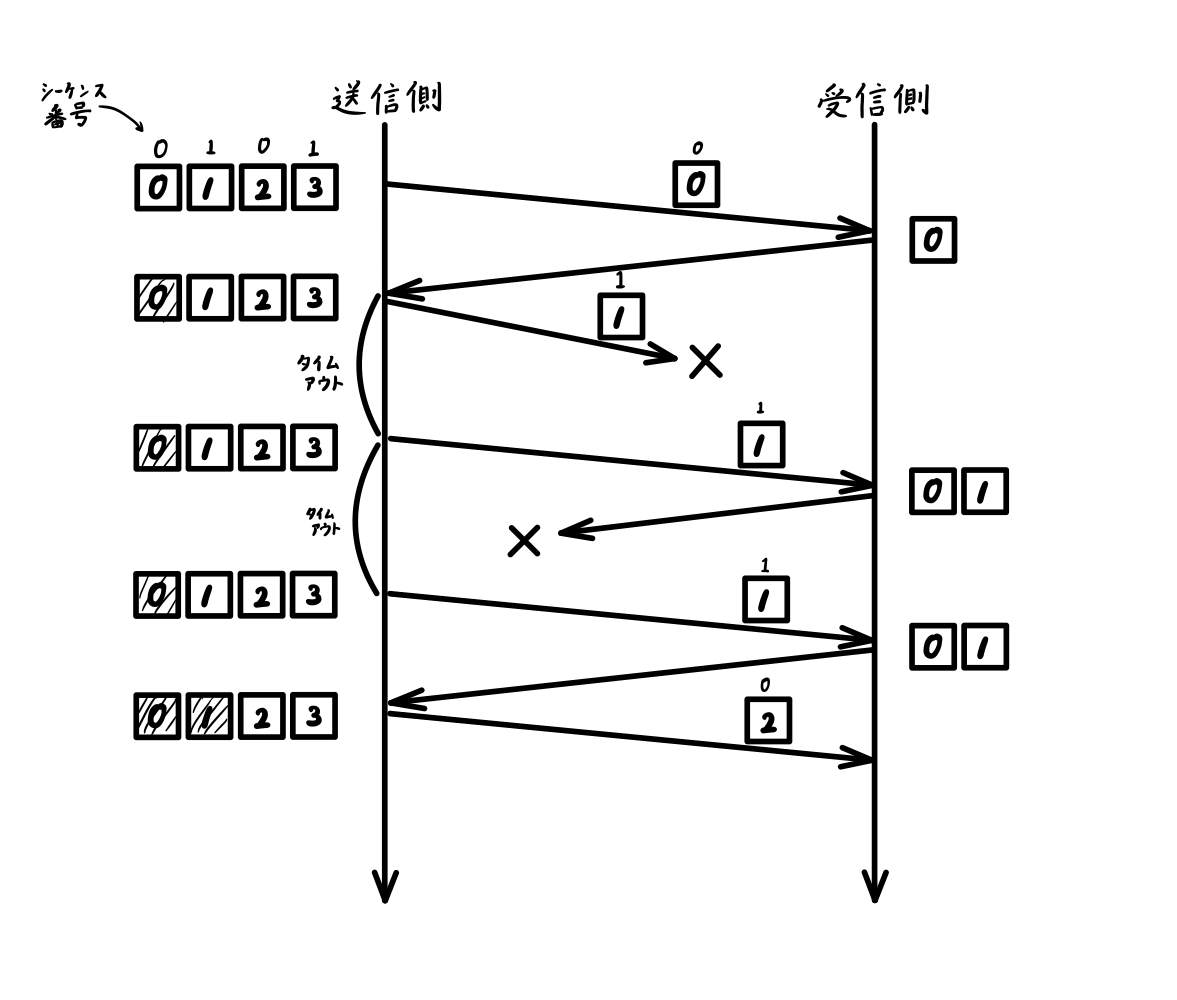
\includegraphics[width=0.65\linewidth]{image/stop_and_wait.png}
\end{figure}

\begin{itemize}
  \item SWの性能の概算
  \begin{itemize}
    \item データパケット長 $L$(bit), 回線速度 $R$ (bit/S), 往復遅延時間 $RTT$ (s)
    \item 1パケットの伝送にかかる時間 $RTT + \frac{L}{R}$
    \begin{itemize}
      \item スループット $\theta = \frac{L}{RTT+\frac{L}{R}}$
      \item 回線利用率 $U = \frac{\theta}{R} = \frac{L}{R \times RTT + L}$
      \item $R\times RTT$: \textcolor{orange}{帯域遅延積(Bandwidth-Delay Product)}
      \item 帯域遅延積が大きくなると回線利用率が低下
      \item[$\rightarrow$] 性能劣化の原因はACK待ちに要する時間
      \item[] \undercolor[black]{パイプライン化}により、性能は向上
    \end{itemize}
  \end{itemize}
\end{itemize}
% SWは大量のデータを流せる回線で使用すると非効率 時間的分割・ラウンドロビンとかRTOSとかに近い感じ?


\subsubsection{Go-back-N (GBN)}

\begin{itemize}
  \item ACKの受信を待たずに、連続するパケットを最大N個まで送信\\
    (スライディングウィンドウプロトコル)
  \item 送信失敗を確認すると、そのパケットから全てやり直し
  \begin{itemize}
    \item 受信した順序が入れ替わっていたら、パケットを捨てる\\
      \textcolor{cyan}{ACKが来ないとウィンドウが進めなくなる}
  \end{itemize}
\end{itemize}
\textcolor{cyan}{受信側が簡単な仕様、TCPはざっくりGo-back-Nだけど、すぐに捨てるわけじゃないみたい}

\begin{figure}[h]
% img 0~6の情報を3つずつ送信してる図
  \centering
  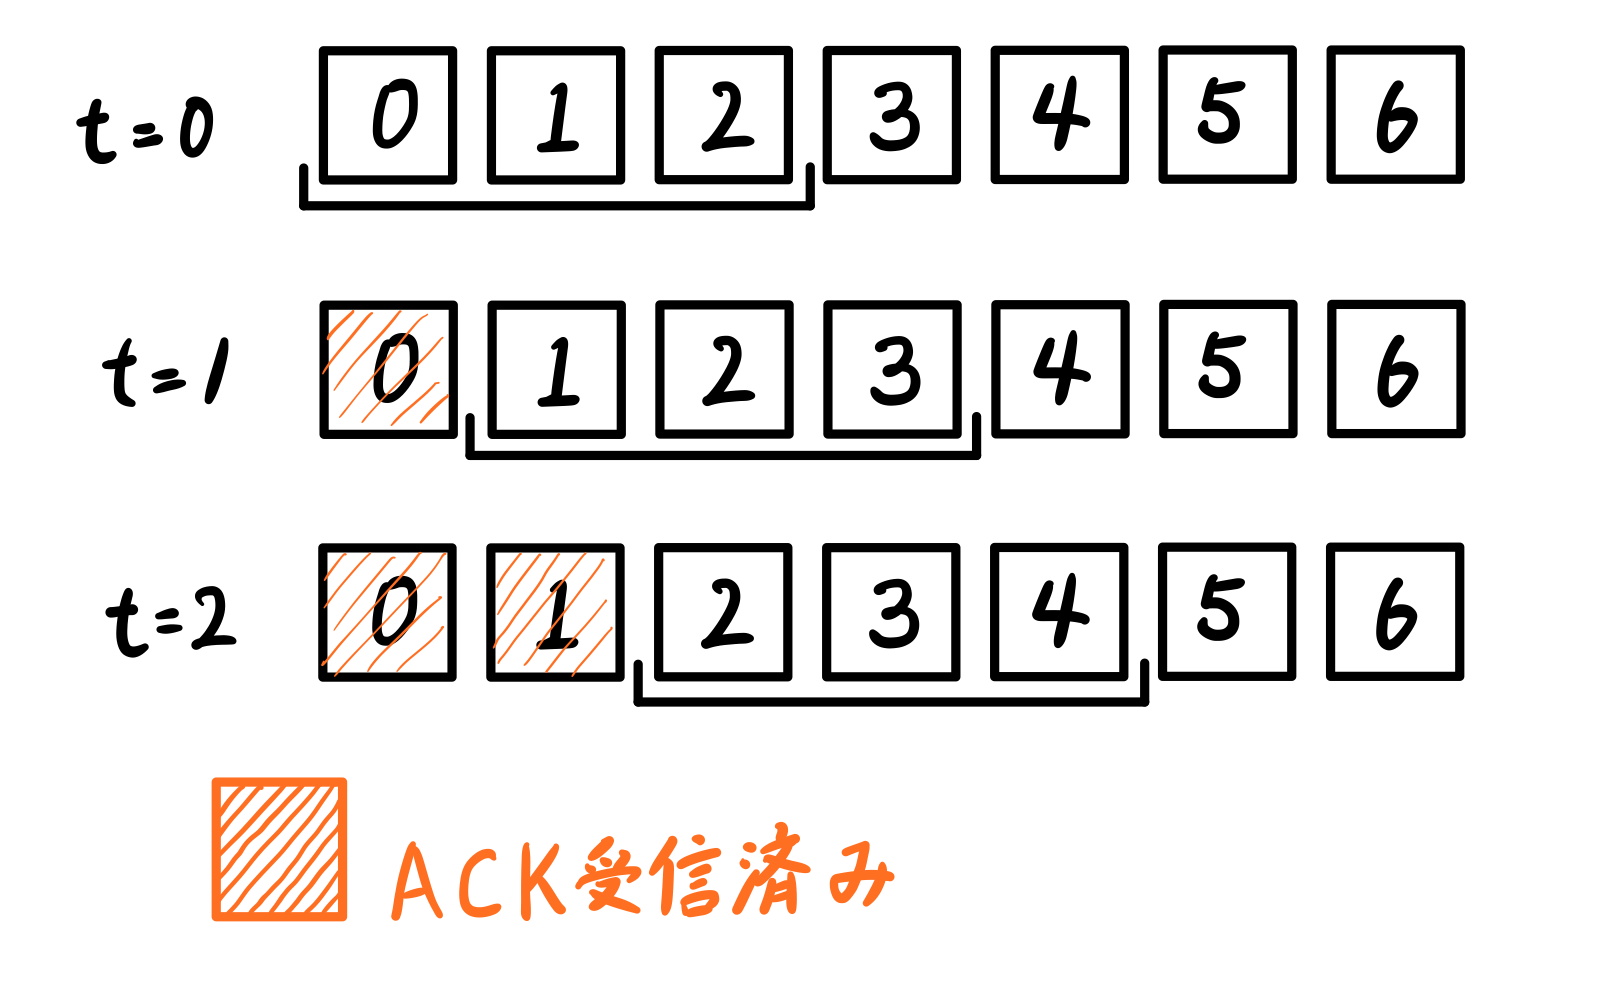
\includegraphics[width=0.4\linewidth]{image/go_back_n.png}
\end{figure}
